% \documentclass[border=0]{standalone}
\documentclass[a3paper]{article}
\usepackage[left=-2mm,top=2mm,right=0mm,bottom=0mm]{geometry}
\usepackage{tikz}
\begin{document}
\thispagestyle{empty}
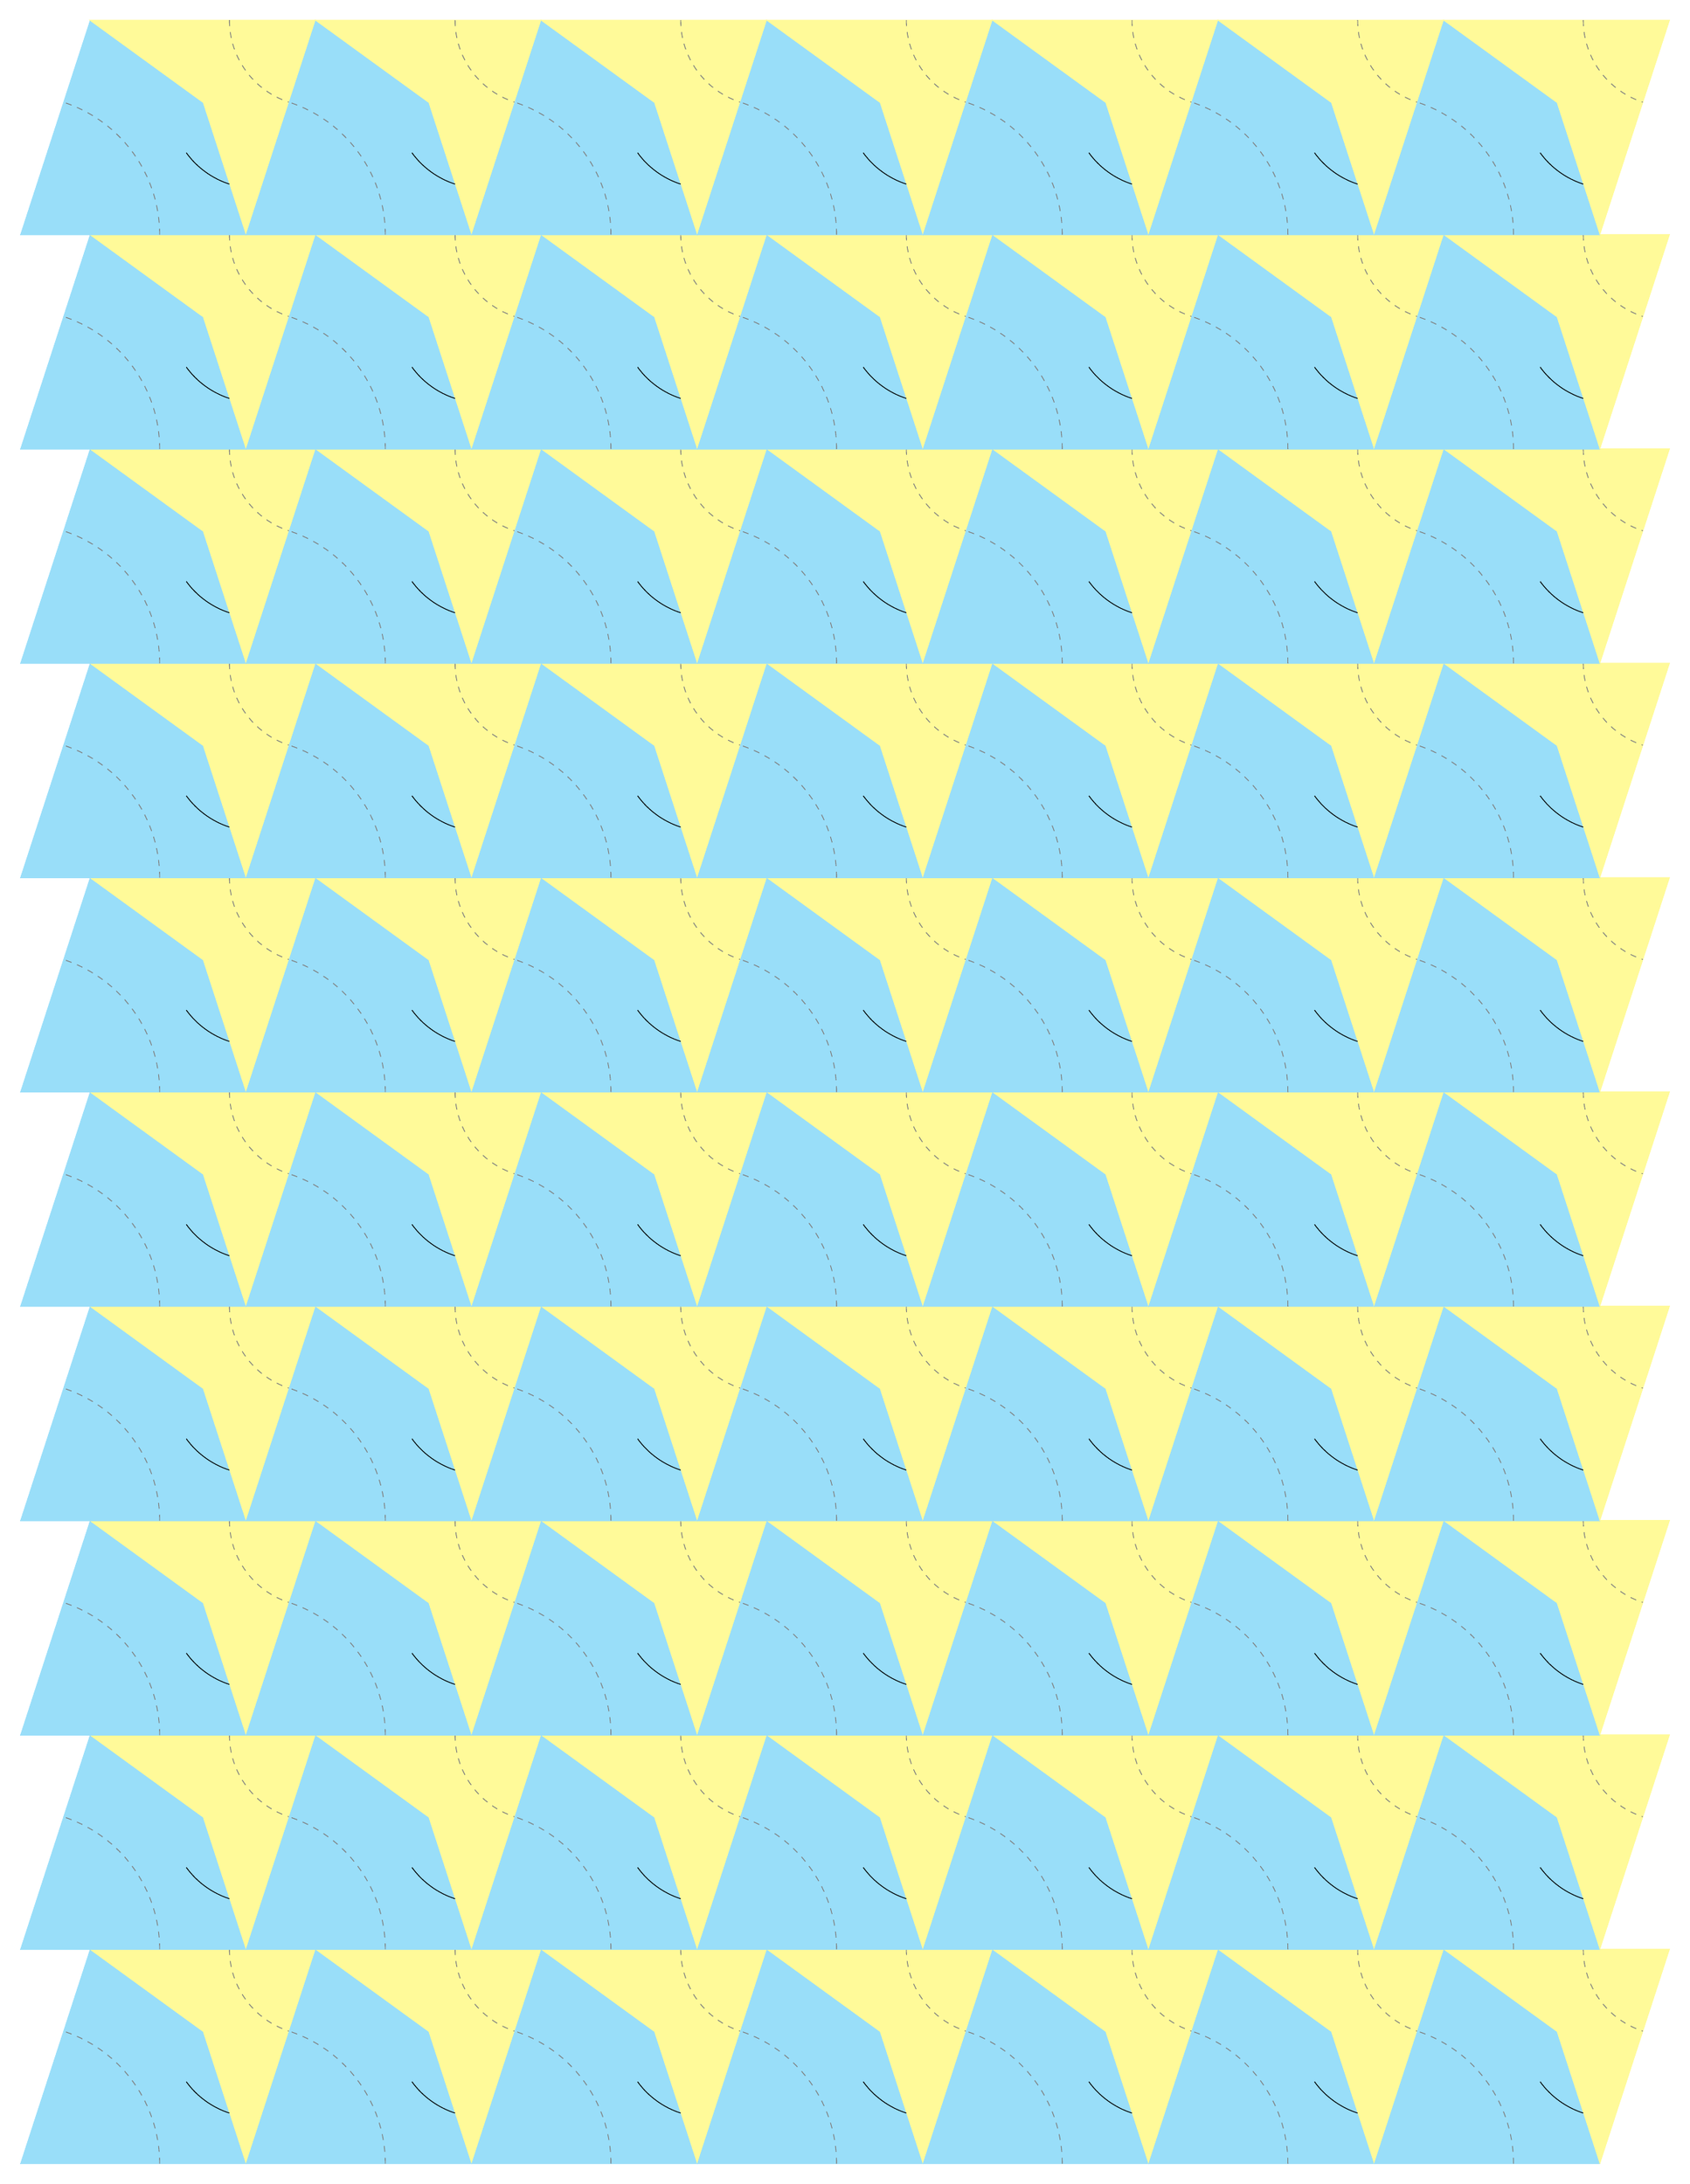
\begin{tikzpicture}
    \pgfmathsetmacro{\p}{(1+sqrt(5))/2}
    \pgfmathsetmacro{\l}{4}
    \foreach \x in {0,1,2,...,6}{
        \foreach \y in {0,1,...,9}{
            \filldraw[cyan!40] (\l*\x,3.8*\y) --++ (0:\l)--++(108:\l/\p)--++(144:\l/\p);
            \filldraw[yellow!40] (\l*\x,3.8*\y) ++ (0:\l) -- ++ (72:\l) --++(180:\l)--++(-36:\l/\p);
            % \draw (4*\x,3.8*\y) --++ (0:4)--++(72:4)--++(180:4)--++(-36:4/\p)--++(-72:4/\p);
            \draw[dashed,gray] (\l*\x,3.8*\y)++(0:{\l*\p/(1+\p)}) arc (0:72:{\l*\p/(1+\p)});
            \draw[dashed,gray] (\l*\x,3.8*\y)++(72:\l)++(0:{\l*\p/(1+\p)}) arc (180:252:{\l/(1+\p)});
            \draw (\l*\x,3.8*\y)++ (0:\l)++(108:{\l/(\p*(\p+1))}) arc (-108:-144:{\l/(\p+1)});
        }
    };

\end{tikzpicture}
\end{document}
    % \draw (0,0)--(0:4)--++(72:4)--++(180:4)--(0,0);
    % \draw (72:4) -- (36:4) -- (0:4)--++(72:4);